\documentclass{article}
\usepackage{graphicx} % Required for inserting images
%\usepackage{geometry}
%\geometry{margin=1in}
\usepackage[margin=1in]{geometry}
\usepackage{algpseudocode}
\usepackage{algorithm}
\usepackage{url}
\usepackage{amsmath, amsthm, amssymb}
\usepackage{booktabs}
\usepackage{pgfplotstable}
\usepackage{tikz-cd}
\usepackage{tikz}
\usetikzlibrary{arrows}
\usepackage{hyperref}
\usepackage{float}

\title{CS4150 Theory 6 Solutions}
\author{Fall 2023}
\date{October 2023}

\begin{document}

\maketitle

\section*{Quiz A}
\subsection*{Question 1}

\textbf{Solution}: We start with $GCD(F_{k+1}, F_k)$ meaning we will recurse to $GCD(F_k, F_{k+1} \% F_k)$. Since $F_{k+1} = F_k + F_{k-1}$, then $F_{k+1} \% F_k = F_{k-1}$. Therefore $GCD(F_k, F_{k+1} \% F_k) = GCD(F_k, F_{k-1})$. We can recursively continue this process until we get to $GCD(F_1, F_0)$ which will return. Since on each level we are decreasing the value of $F_k$ by one, we end up with $k$ iterations.

\subsection*{Question 2}
\textbf{Solution:} Consider if $d > 1$. Then $GCD(x,y) = d \Rightarrow d | x \text{ and } d | y$. This implies we can rewrite $x = d\cdot q$ and $y = d \cdot q'$. By substituting these in to the equation $x \equiv 1 \mod y$ to get $d\cdot q \equiv 1 \mod d\cdot q'$. Then it must mean that $dq = dq'z + 1, z \in \mathrm{Z}^+$. Let $z = 1$, then $ dq - dq' = 1 \Rightarrow d\cdot(q-q') = 1$. Since $d,q,q' \in \mathrm{Z}^+$, it must be that $q-q' = d = 1$. However, this contradicts our original statement that $d > 1$. Therefore, it must be true that: If $x \equiv 1 \mod y \Rightarrow GCD(x,y)=1$

\subsection*{Question 3}
\textbf{Solution:}
\subsubsection*{i)} If $a \equiv b \mod N \text{ and } x \equiv y \mod N$, then since both are $\mod N$ they adhere to normal rules of multiplication, meaning we may write $ax\equiv by \mod N$.
\subsubsection*{ii)} False with counter example $a = 2, b = 2, x = 7, y = 2, N = 5$. Note that $2 \equiv 2 \mod 5$ and $7 \equiv 2 \mod 5$ but $2^7 \not\equiv 2^2 \mod 5 \Rightarrow 3 \not\equiv 4 \mod 5$

\subsection*{Question 4}
\textbf{Solution:} Consider $(X+Y) \cdot (X-Y)$. If we expand we get $X^2 + Y^2 + XY - XY = X^2 + Y^2$. Since we can find squares in $O(n)$ time, we do $2\cdot O(n) = O(n)$ operations to multiply numbers $(X+Y)$ and $(X-Y)$. Therefore we have done better than $O(n \cdot \log^3(n))$. Note: a cool generalization of this is that for any number $J$, $J$ can be factored into computations involving only squares or additions. 

\subsection*{Question 5}
\textbf{Solution:} Let $a = 3, b = 6$. $ab \equiv 0 \mod 18 \Rightarrow 18 \equiv 0 \mod 18$, but $3 \not\equiv 0 \mod 18$ and $6 \not\equiv 0 \mod 18$

\subsection*{Question 6}
\textbf{Solution} Since $GCD(c,N) = 1$ then $c$ and $N$ are co-prime. This means by the cancellation law of congruence: $cx \equiv cy \mod n \Rightarrow x \equiv y \mod n$\\

\noindent \textbf{Alternate Solution} $cx \equiv cy \mod N \Rightarrow cx-cy \equiv 0 \mod N \Rightarrow c(x-y) \equiv 0 \mod N \Rightarrow N | c(x-y)$. If $GCD(c,N) = 1$, then $c$ and $N$ don't share any factors, meaning if $N|c(x-y) \Rightarrow N|(x-y)$ since $x-y$ must be some multiple of $N$. $N|(x-y) \Rightarrow x-y \equiv 0 \mod N \Rightarrow x \equiv y \mod N$\\ 

\noindent \textbf{Theorem:} Cancellation Law of Congruence \\
$ca \equiv cb \mod n \Rightarrow a \equiv b \mod \frac{n}{d}$ where $d = gcd(c,n)$.\\

    \noindent$pf.$\\
    $n | ca-cb \Rightarrow ca-cb = qn, \exists q \in \mathrm{Z} (*)$\\
    $\Rightarrow c(a-b) = qn, \exists q \in \mathrm{Z}$\\
    $\text{From the hypothesis } d = gcd(c,n)$\\
    $c = dr \text{ and } n = ds \text{ with } gcd(r,s) = 1 (**)$\\
    $\text{ plugging $*$ into $**$ we get } dr(a-b) = qds$\\
    $\Rightarrow r(a-b) = qs \text{ since } gcd(r,s) = 1$\\
    $\Rightarrow s | (a-b) \text{ by Euclid's lemma ($a | bc \text{ and } gcd(a,b)=1 \Rightarrow a|c$) }$\\
    $\Rightarrow a \equiv b \mod s \text{ (since } n = ds \Rightarrow s = \frac{n}{d} \text{)}$\\
    $\Rightarrow a \equiv b \mod \frac{n}{d}$


\subsection*{Question 7}
\textbf{Solution:} Since $N \equiv 7 \mod 11$ then $N = 11k + 7$. Try integers $k = 1\rightarrow 20$ until one works for both equations. $k = 11$ works, $N = 11\cdot 11 + 7 = 128$. Then $128 \equiv 7 \mod 11$ and $128 \equiv 11 \mod 13$ (note that $13*9 = 117 \Rightarrow 128 - 117 = 11$)

\subsection*{Question 8}
\textbf{Solution:} 
\subsubsection*{a)} If one digit is incorrect we will be off by some number $i \in [0,9]$ which all have unique values $\mod 11$. Therefore, the total sum is off by $|a_i-i| \leq 9$ which will have unique value $\mod 11$.

\subsection*{b)} If two indices are swapped and produce the same result then $a_i + 2a_{i+1} \equiv a_{i+1} + 2a_i \mod 11$. If we rearrange the equation to get $a_i + 2a_{i+1} - (a_{i+1} + 2a_i) \equiv 0 \mod 11 \Rightarrow a_{i+1} - a_i \equiv 0 \mod 11$. However, note that the largest value that $a_{i+1} - a_i$ can be is 9, and since $GCD(11, 9) = 1$, then there can only be unique values for the sum if two numbers are swapped.

\section*{Quiz B}
\subsection*{Question 1}
\textbf{Solution:} $x^2 \equiv 1 \mod p \Rightarrow x^2 - 1 \equiv 0 \mod p \Rightarrow (x+1)\cdot (x-1) \equiv 0 \mod p$. From Quiz A, we know that iff $ab \equiv 0 \mod p \Rightarrow a \equiv 0 \mod p$ and $b \equiv 0 \mod p$. Therefore, $(x+1)\cdot (x-1) \equiv 0 \mod p \Rightarrow (x+1) \equiv 0 \mod p$ and $(x-1)\equiv 0 \mod p$. Let's start with $(x-1)\equiv 0 \mod p \Rightarrow x \equiv 1 \mod p$. Since $x < p$ the only value that satisfies this equation is $x = 1$. Now for $(x+1) \equiv 0 \mod p \Rightarrow x \equiv -1 \mod p$, but we can't have $x$ be equivalent to a negative modulo a number, so we take the next common multiple (just add the modulus to the negative until it is positive). This means that $x \equiv -1 + p \mod p \Rightarrow x \equiv p-1 \mod p$. Similarly as before, since $x < p$ the only value that satisfies this equation is $x = p-1$ 

\subsection*{Question 2}
\textbf{Solution:} Drawing a graph with and $p=7$ 

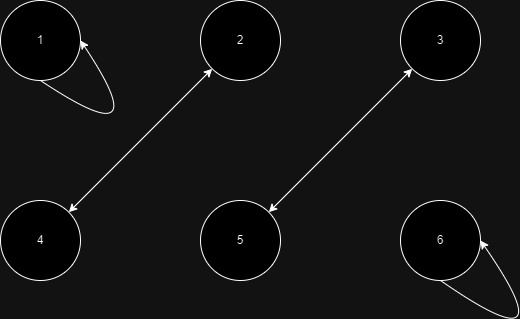
\includegraphics[scale=0.5]{graph.jpg}
\newpage
\subsection*{Question 3}
\textbf{Solution:} $(p-1)! \equiv p-1 \mod p \Rightarrow 1\cdot 2 \cdot \ldots \cdot (p-2) \cdot (p-1) \equiv p-1 \mod p$. Note that in the previous question we saw that the only numbers who don't have inverses were $1$ and $p-1$. This means all values $2, \ldots, p-2$ will have an inverse with another number in range $[2, p-2]$. This means that $1\cdot 2 \cdot \ldots \cdot (p-2) \cdot (p-1) \equiv p-1 \mod p \Rightarrow 1\cdot (p-1) \cdot \prod_{i=1}^{k =\frac{p-3}{2}}1 \equiv p-1 \mod p \Rightarrow p-1 \equiv p-1 \mod p$.

\subsection*{Question 4}
\textbf{Solution:} Note that if $N$ is composite, there exist some factors $ab = N$
\subsubsection*{Case $a=b$} If $a=b \Rightarrow a^2 = N \equiv 0 \mod N$. Now, note that $a^2-a$ is a multiple of $a$, which means $a^2-a \equiv 0 \mod N$. Given our original equation: $(N-1)! \equiv 0 \mod N \Rightarrow 1\cdot 2\cdot \ldots \cdot (a-1) \cdot a \cdot \ldots \cdot (N-1) \equiv 0 \mod N$. Then we can pull $(a-1)\cdot a = a^2 -a$ out of the expression to get $(a^2-a) \cdot [1\cdot \ldots \cdot (a-2)\cdot (a+1) \cdot \ldots \cdot (N-1)] \equiv 0 \mod N$. Note that any multiple of $a^2-a \equiv 0 \mod N$, so if we let $k = 1\cdot \ldots \cdot (a-2)\cdot (a+1) \cdot \ldots \cdot (N-1)$, then $(a^2-a)\cdot k \equiv 0 \mod N$.

\subsubsection*{Case $a\neq b$} This case follows similar logic, since $a < N$ and $b < N$, then $a,b \in [1, N-1]$. Therefore, $(N-1)! \equiv 0 \mod N \Rightarrow 1\cdot \ldots \cdot a \cdot b \cdot \ldots \cdot (N-1) \equiv 0 \mod N \Rightarrow a\cdot b \cdot [1\cdot \ldots (a-1) \cdot (b+1) \cdot \ldots \cdot (N-1)] \equiv 0 \mod N$. Let $k = 1 \cdot \ldots (a-1) \cdot (b+1) \cdot \ldots \cdot (N-1)$. Then, $a\cdot b \cdot k \equiv 0 \mod N$ since $ab = N$ and any multiple of $N$ will satisfy the equation. \\ 

\noindent Therefore, by cases $a=b$ and $a\neq b$, we have shown $(N-1)! \equiv 0 \mod N$ if $N > 4$ and $N$ is composite.

\subsection*{Question 5}
\textbf{Solution:} This will be very slow and resource intensive for large numbers. For example RSA uses numbers that are $4096$ bits. This means that we would have to calculate $(2^{4096})!$ which is not efficient at all. A probabilistic test will be much faster with a high probability of success. \\

\noindent Fun note: For example Fermat's test $a^{p-1} \equiv 1 \mod p$ can be done for $10$ primes will probability of failure $< \frac{1}{2^{10}}$ meaning the probability of success is $ > 1 - \frac{1}{2^{10}} = 0.9990234375$

\end{document}
 